\documentclass{minimal}
\usepackage{tikz}
\usetikzlibrary{external, calc, positioning, arrows.meta}

%\tikzexternalize

\begin{document}
	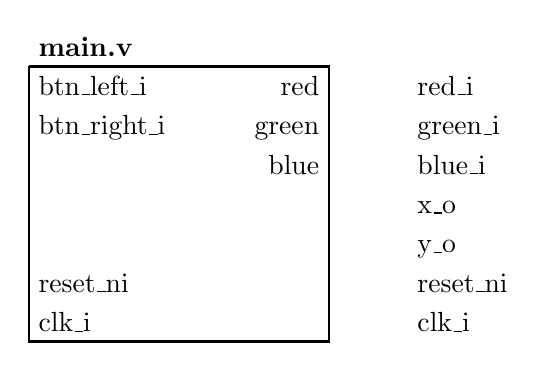
\begin{tikzpicture}

		% main.v
		\node[anchor=west] (btnleft){btn\_left\_i};
		\node[below=5mm of btnleft.base west,anchor=base west] (btnright){btn\_right\_i};

		\node[below=20mm of btnright.base west,anchor=base west] (resetnim){reset\_ni};
		\node[below=5mm of resetnim.base west,anchor=base west] (clkinm){clk\_i};

		\node[right=30mm of btnleft.base,anchor=base east,align=left]
			(red){red};
		\node[below=5mm of red.base east,anchor=base east,align=left]
			(green){green};
		\node[below=5mm of green.base east,anchor=base east,align=left]
			(blue){blue};

		\draw[thick] (btnleft.north west)--(clkinm.south west)
			-- (clkinm.south west -| red.north east)
			-- (red.north east) -- (btnleft.north west);
		\node[above=5mm of btnleft.base west,anchor=base west](mainv){\textbf{main.v}};

		% vga.v
		\node[right=10mm of red.base east,anchor=base west](redi){red\_i};
		\node[below=5mm of redi.base west,anchor=base west](greeni){green\_i};
		\node[below=5mm of greeni.base west,anchor=base west](bluei){blue\_i};

		\node[below=5mm of bluei.base west,anchor=base west](xo){x\_o};
		\node[below=5mm of xo.base west,anchor=base west](yo){y\_o};

		\node[below=20mm of greeni.base west,anchor=base west](resetniv){reset\_ni};
		\node[below=5mm of resetniv.base west,anchor=base west](clkiv){clk\_i};


	\end{tikzpicture}
\end{document}
